\documentclass[11pt, a4paper]{article}
\usepackage{pdfpages}
\usepackage{parallel}
\usepackage[T2A]{fontenc}
\usepackage{ucs}
\usepackage[utf8x]{inputenc}
\usepackage[polish,english,russian]{babel}
\usepackage{hyperref}
\usepackage{rotating}
\usepackage[inner=2cm,top=1.8cm,outer=2cm,bottom=2.3cm,nohead]{geometry}
\usepackage{listings}
\usepackage{graphicx}
\usepackage{wrapfig}
\usepackage{longtable}
\usepackage{indentfirst}
\usepackage{array}
\usepackage{tikzsymbols}
\usepackage{soul}
\usepackage[ruled,vlined]{algorithm2e}
%\counterwithout{figure}{section} 

\usepackage{url}
\makeatletter
\g@addto@macro{\UrlBreaks}{\UrlOrds}
\makeatother

\newcolumntype{P}[1]{>{\raggedright\arraybackslash}p{#1}}
\frenchspacing
\usepackage{fixltx2e} %text sub- and superscripts
\usepackage{icomma} % коскі ў матэматычным рэжыме
\PreloadUnicodePage{4}

\newcommand{\longpage}{\enlargethispage{\baselineskip}}
\newcommand{\shortpage}{\enlargethispage{-\baselineskip}}

\def\switchlang#1{\expandafter\csname switchlang#1\endcsname}
\def\switchlangbe{
\let\saverefname=\refname%
\def\refname{Літаратура}%
\def\figurename{Іл.}%
}
\def\switchlangen{
\let\saverefname=\refname%
\def\refname{References}%
\def\figurename{Fig.}%
}
\def\switchlangru{
\let\saverefname=\refname%
\let\savefigurename=\figurename%
\def\refname{Литература}%
\def\figurename{Рис.}%
}

\hyphenation{admi-ni-stra-tive}
\hyphenation{ex-pe-ri-ence}
\hyphenation{fle-xi-bi-li-ty}
\hyphenation{Py-thon}
\hyphenation{ma-the-ma-ti-cal}
\hyphenation{re-ported}
\hyphenation{imp-le-menta-tions}
\hyphenation{pro-vides}
\hyphenation{en-gi-neering}
\hyphenation{com-pa-ti-bi-li-ty}
\hyphenation{im-pos-sible}
\hyphenation{desk-top}
\hyphenation{elec-tro-nic}
\hyphenation{com-pa-ny}
\hyphenation{de-ve-lop-ment}
\hyphenation{de-ve-loping}
\hyphenation{de-ve-lop}
\hyphenation{da-ta-ba-se}
\hyphenation{plat-forms}
\hyphenation{or-ga-ni-za-tion}
\hyphenation{pro-gramming}
\hyphenation{in-stru-ments}
\hyphenation{Li-nux}
\hyphenation{sour-ce}
\hyphenation{en-vi-ron-ment}
\hyphenation{Te-le-pathy}
\hyphenation{Li-nux-ov-ka}
\hyphenation{Open-BSD}
\hyphenation{Free-BSD}
\hyphenation{men-ti-on-ed}
\hyphenation{app-li-ca-tion}

\def\progref!#1!{\texttt{#1}}
\renewcommand{\arraystretch}{2} %Іначай формулы ў матрыцы зліпаюцца з лініямі
\usepackage{array}

\def\interview #1 (#2), #3, #4, #5\par{

\section[#1, #3, #4]{#1 -- #3, #4}
\def\qname{LVEE}
\def\aname{#1}
\def\q ##1\par{{\noindent \bf \qname: ##1 }\par}
\def\a{{\noindent \bf \aname: } \def\qname{L}\def\aname{#2}}
}

\def\interview* #1 (#2), #3, #4, #5\par{

\section*{#1\\{\small\rm #3, #4. #5}}
\ifx\ParallelWhichBox\undefined%
    \addcontentsline{toc}{section}{#1, #3, #4}%
\else%
\ifnum\ParallelWhichBox=0%
    \addcontentsline{toc}{section}{#1, #3, #4}%
\fi\fi%

\def\qname{LVEE}
\def\aname{#1}
\def\q ##1\par{{\noindent \bf \qname: ##1 }\par}
\def\a{{\noindent \bf \aname: } \def\qname{L}\def\aname{#2}}
}

\newcommand{\interviewfooter}[1]{
\vskip 1em
\noindent \textit{#1}
}


\begin{document}

\title{1983 "--- Logitech LOGIMOUSE P5}
\date{}
\maketitle

LOGIMOUSE P5 mouse was released in 1983. This is the second manipulator from Logitech (after the famous  P4 mouse, production of which continued simultaneously with P5). LOGIMOUSE P5 was a cheaper model (the selling price differed by \$100), and it was intended primarily for OEM supplies. But the main feature of the P5 is a radically different exterior (fig. \ref{fig:LogimouseP5Pic}).

\begin{figure}[h]
   \centering
    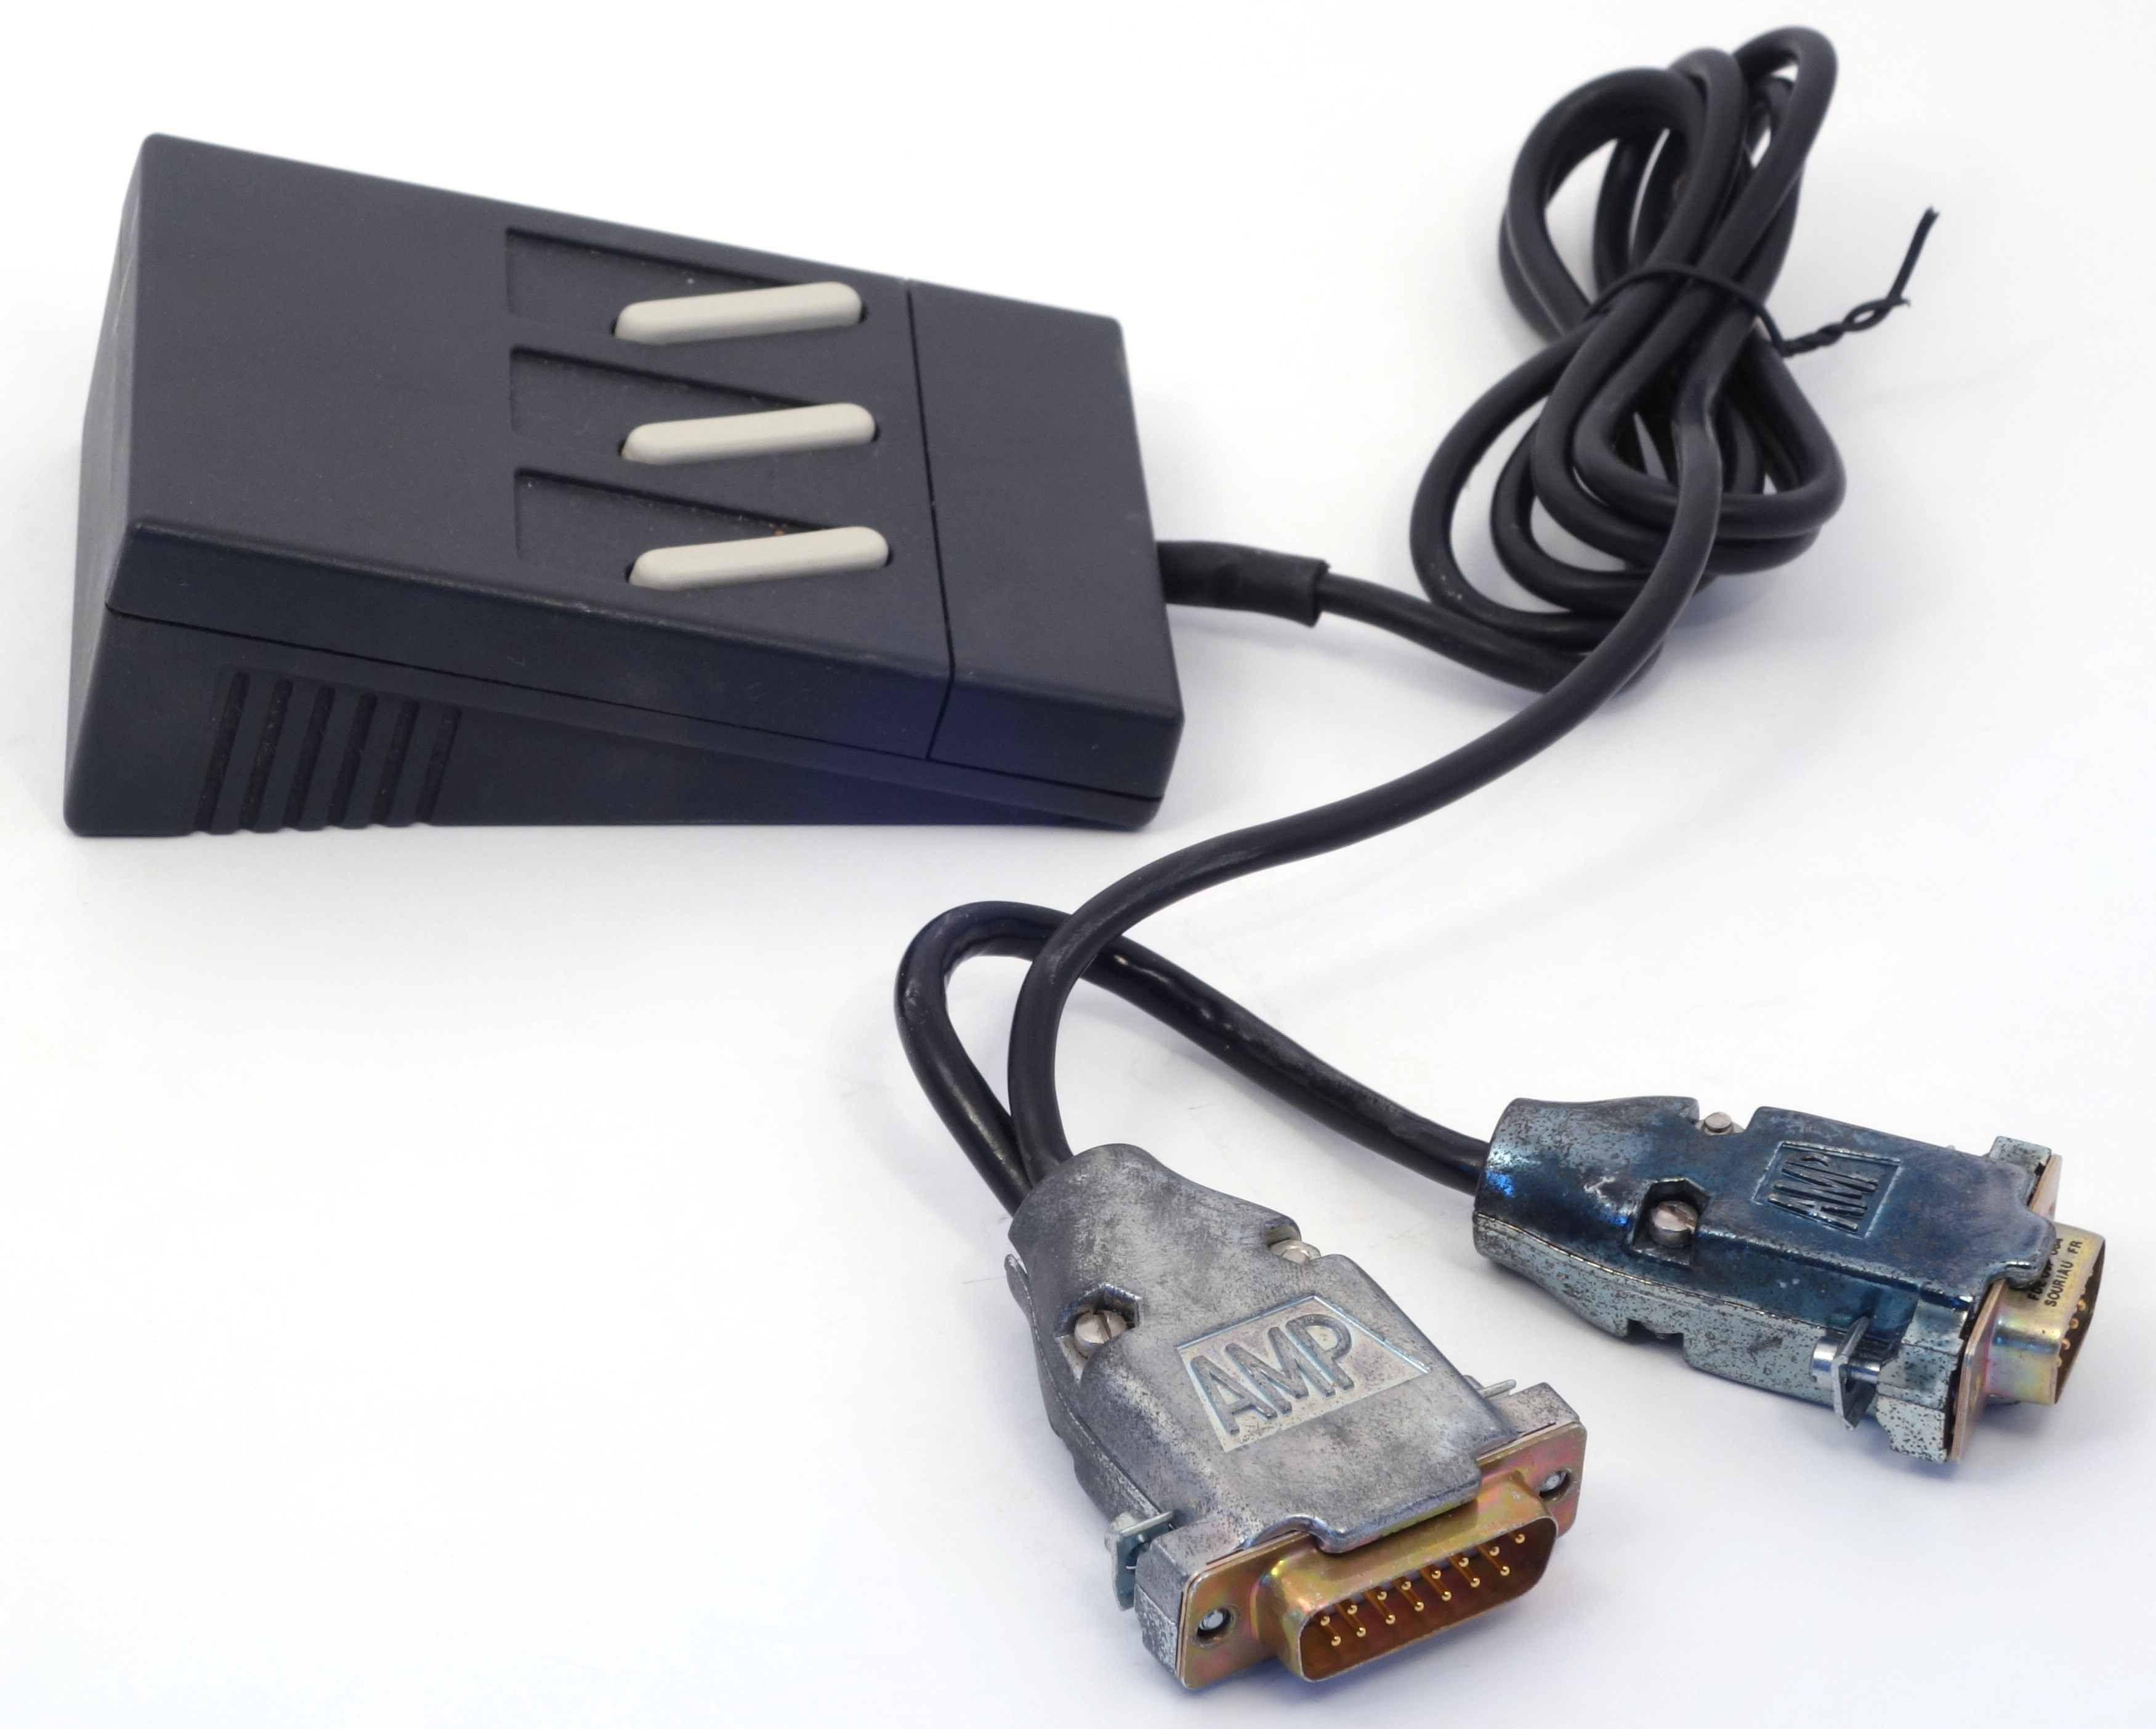
\includegraphics[scale=0.35]{1983_logitech_logimouse_p5/pic_30.jpg}
    \caption{LOGIMOUSE P5}
    \label{fig:LogimouseP5Pic}
\end{figure}

The mouse has a defiant design look, although in 1983 this concept did not yet exist in relation to mice: three narrow white buttons are placed diagonally on a black prismatic body with a reverse slope. On the underside, there are four low-friction white supports (which are also PCB mounts) and a brushed metal ball (fig. \ref{fig:LogimouseP5TopAndBottom}). A removable turnable ring with latches allows you to remove the ball to get rid of accumulated dirt and to clean the rollers. Logitech P4 and other mice of the first half of the 80s did not have a ring or it had to be unscrewed with a screwdriver. Therefore, P5 is one of the first cases (along with the Apple Lisa mouse released in the same year) to use this turnable ring, which later became the standard.

\begin{figure}[h]
    \centering
    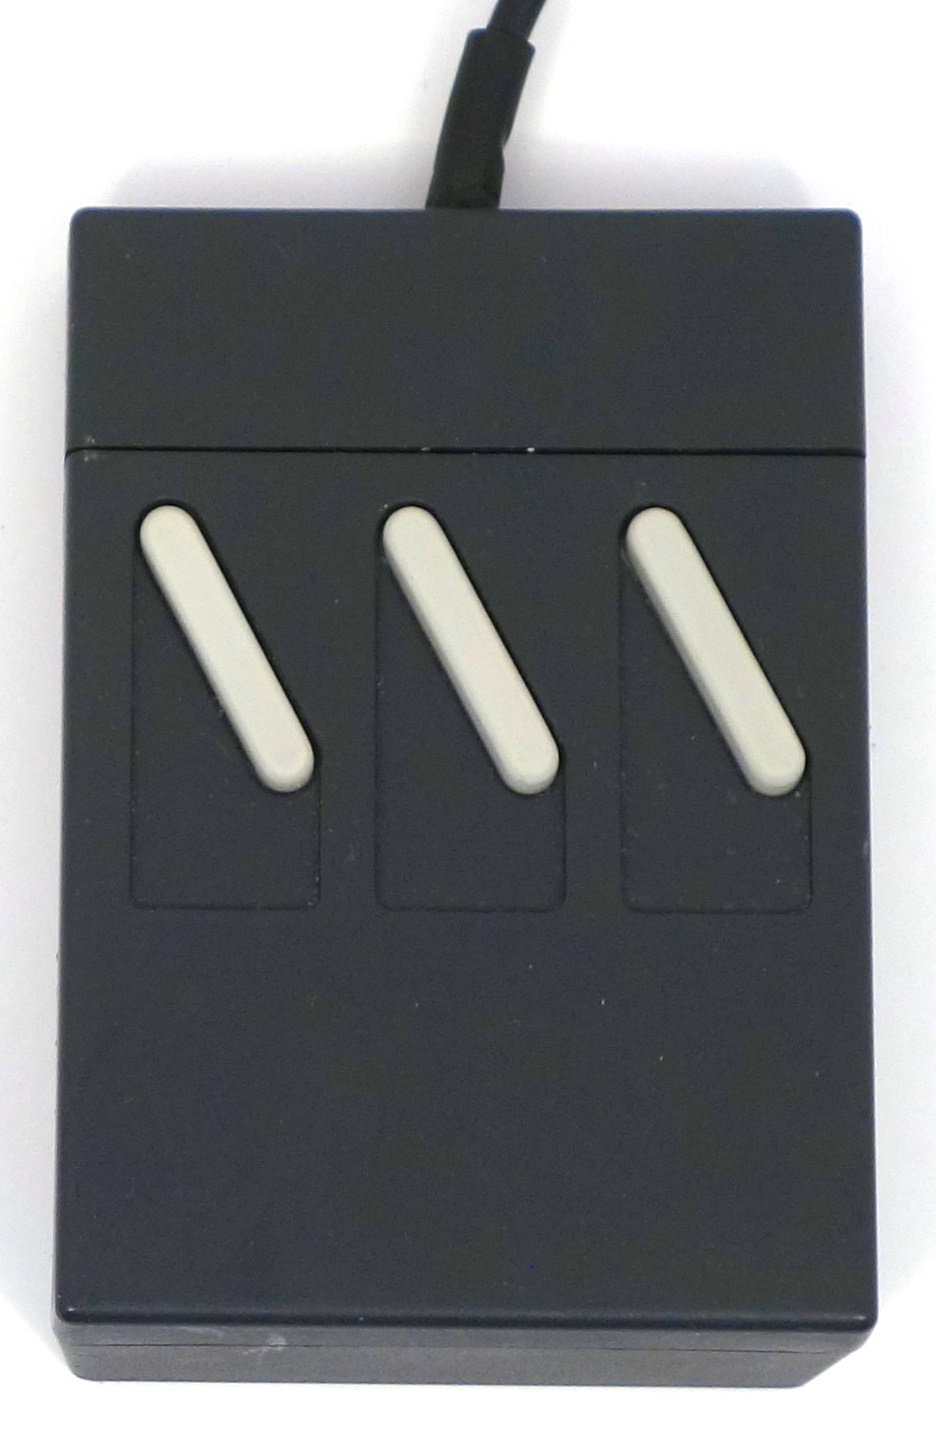
\includegraphics[scale=0.4]{1983_logitech_logimouse_p5/top_30.jpg}
    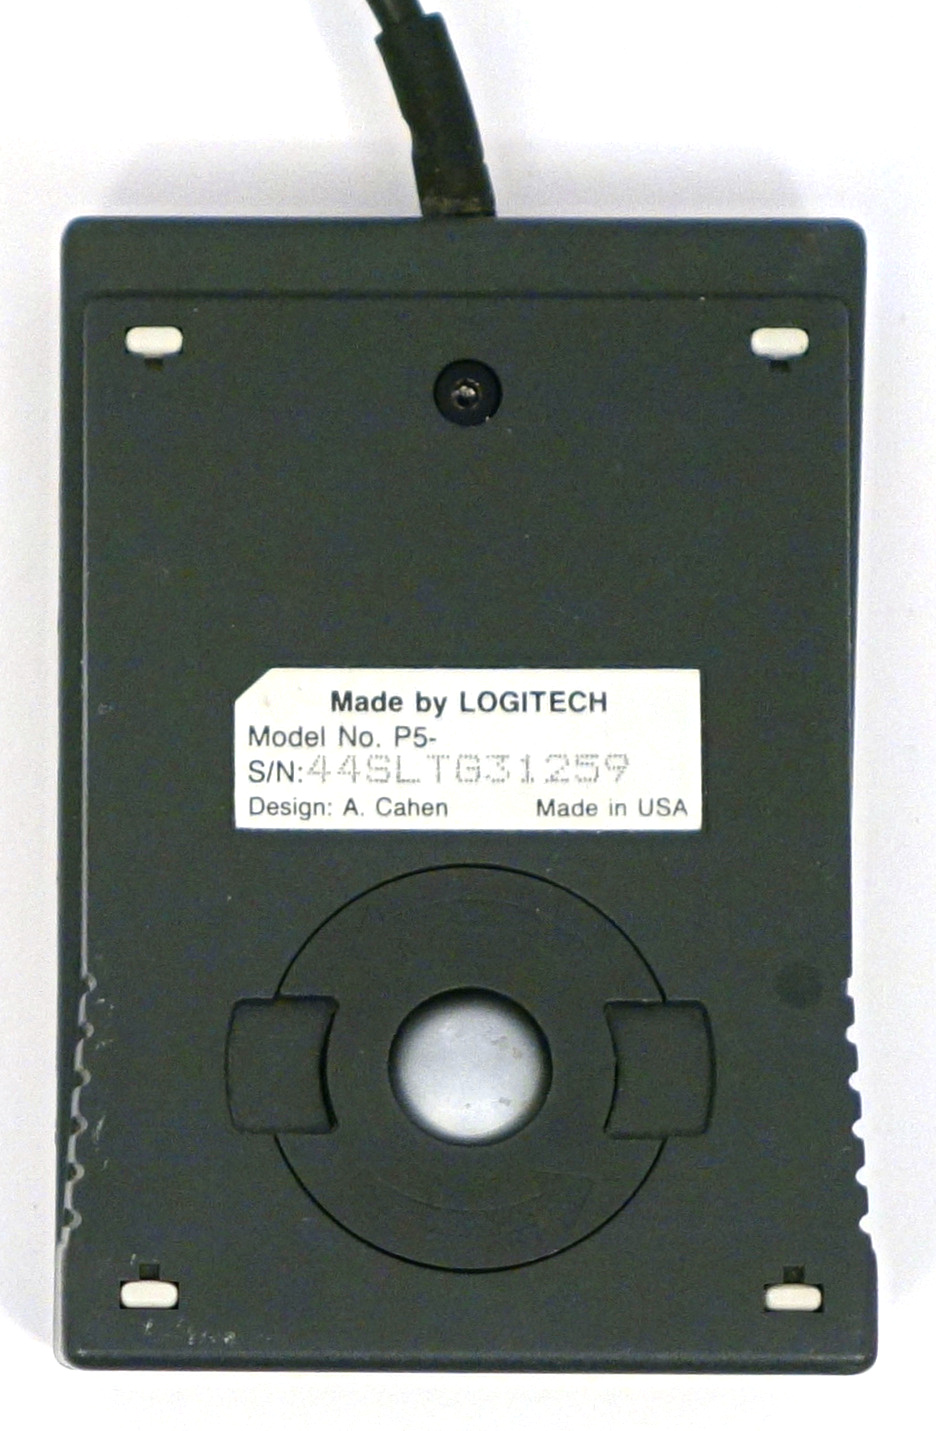
\includegraphics[scale=0.4]{1983_logitech_logimouse_p5/bottom_30.jpg}
    \caption{LOGIMOUSE P5, top and bottom views}
    \label{fig:LogimouseP5TopAndBottom}
\end{figure}

Judging by the cable with two connectors, this is a mouse from FutureNet "---a workstation for microelectronics CAD. This computer was a classic IBM PC with a monochrome text video adapter and an additional graphics card with a resolution of 640x360 pixels, and the fifteen-pin connector on the mouse cable was used to to connect the output of an IBM monochrome video adapter to a graphics card. This allowed the display to be used alternately for text output and for graphics output by the schematic editor \cite{futurenet}.

\begin{figure}[h]
    \centering
    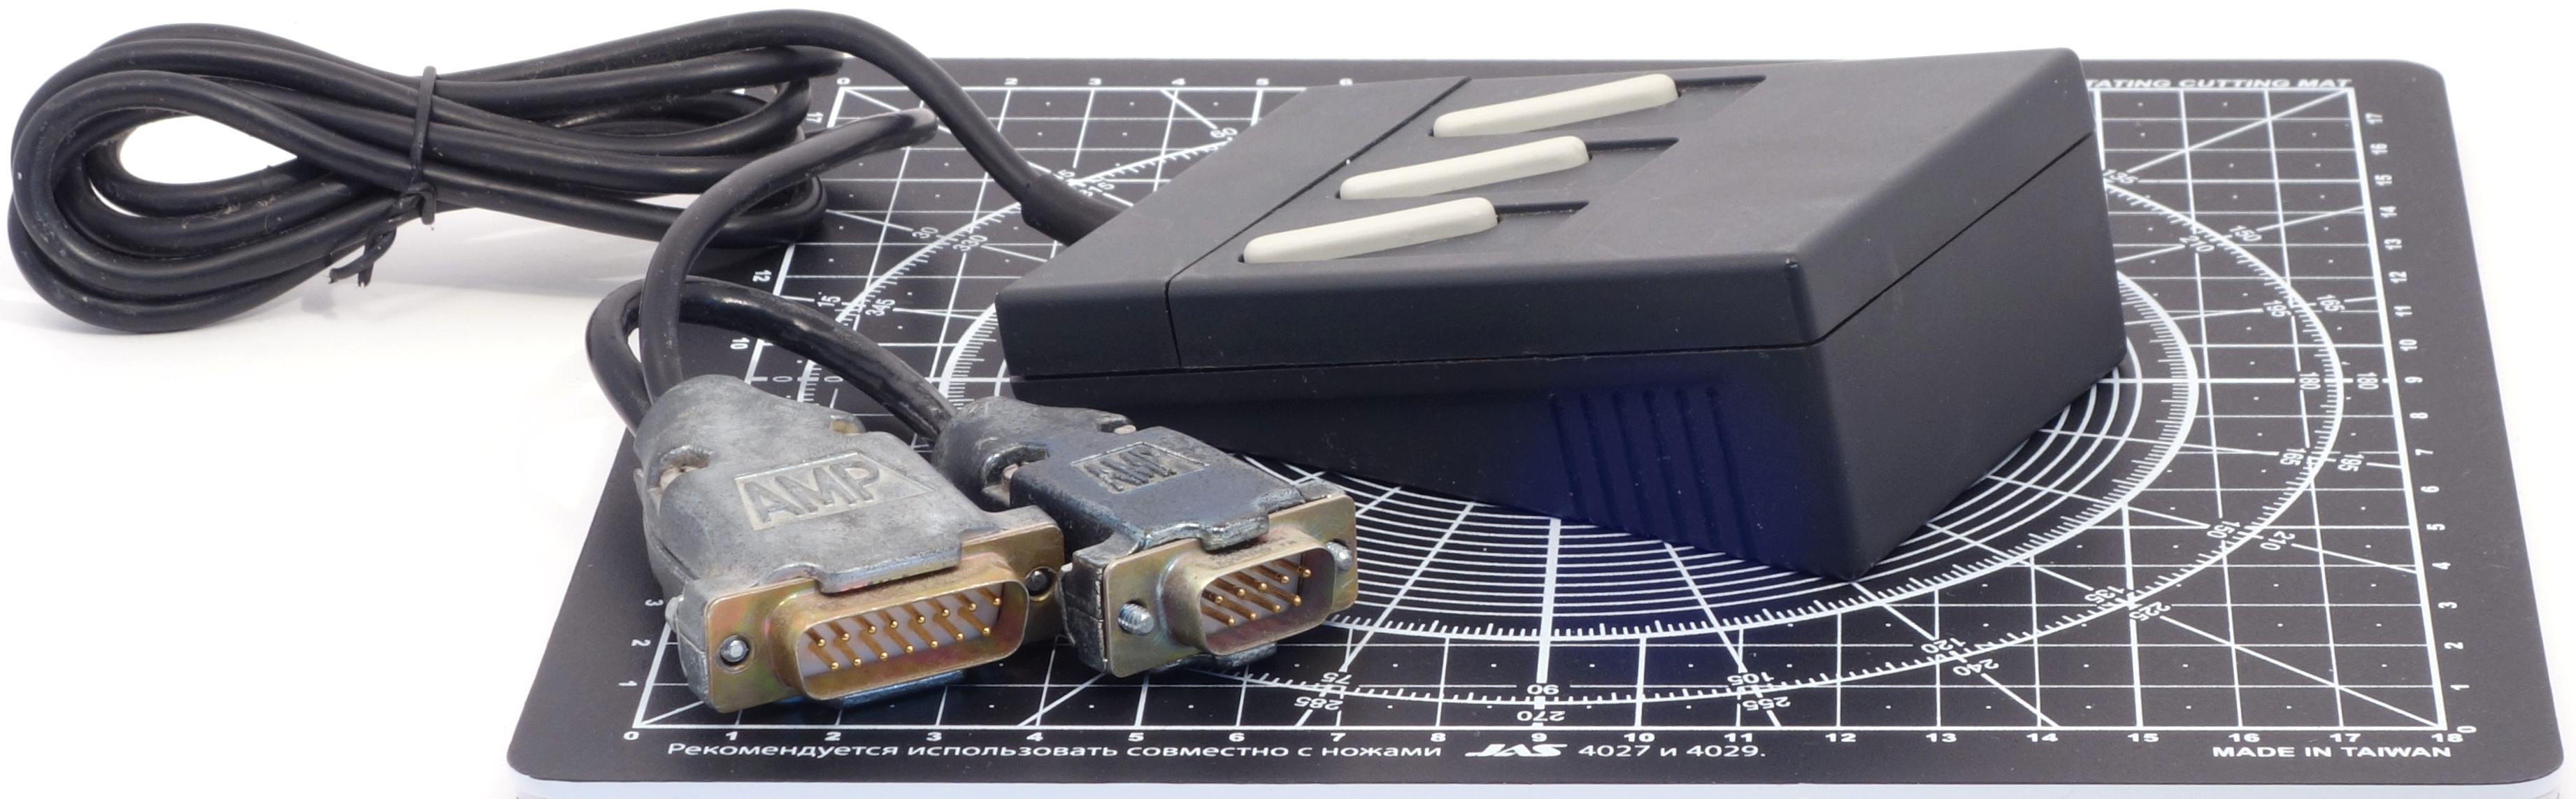
\includegraphics[scale=0.5]{1983_logitech_logimouse_p5/size_30.jpg}
    \caption{LOGIMOUSE P5 on a graduated pad with a grid step of 1~cm}
    \label{fig:LogimouseP5Size}
\end{figure}

The size of the mouse is typical for mice from the 1980s (fig. \ref{fig:LogimouseP5Size}). In fact, its dimensions are close to the later Logitech P7 and its most mass-produced variant, the C7. As for ergonomics, it is obvious that the prismatic case and diagonal narrow buttons had a very negative effect: when placing fingers along the buttons, the palm runs the risk of leaning on the protruding corner of the case; placing the palm along the lines of the body improves the situation only slightly, instead making it more difficult to press the already inconvenient buttons (Fig. \ref{fig:LogimouseP5Hand}).

\begin{figure}[h]
    \centering
    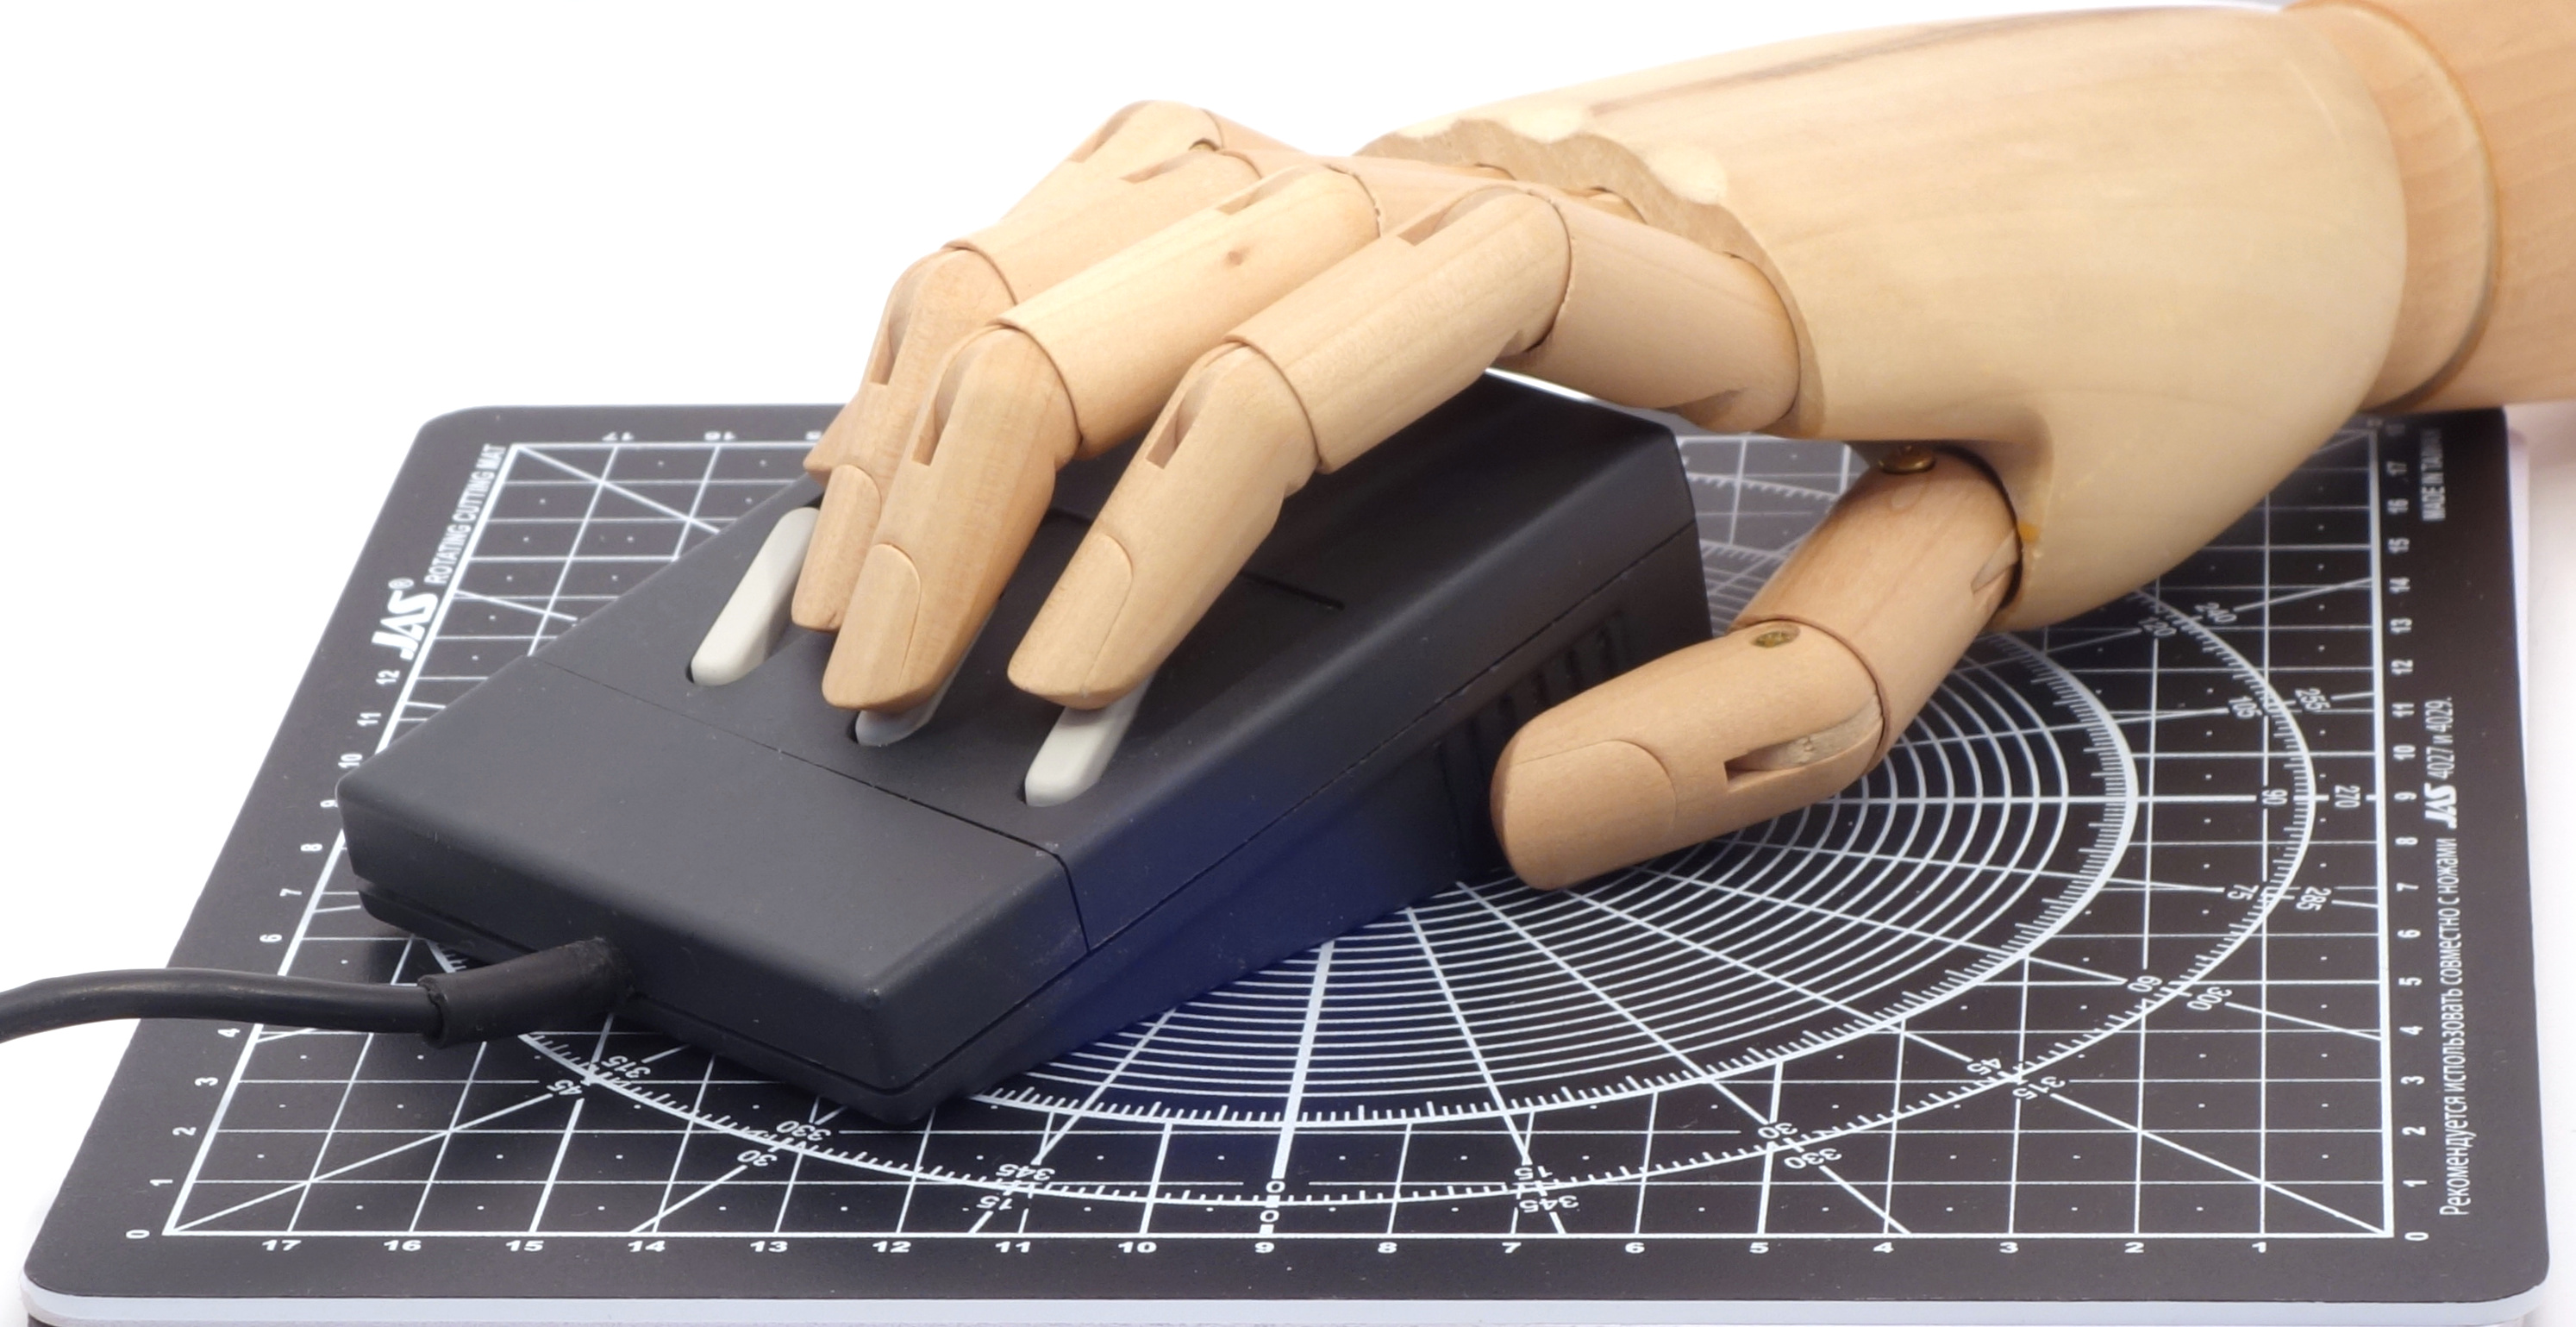
\includegraphics[scale=0.5]{1983_logitech_logimouse_p5/hand_30.jpg}
    \caption{LOGIMOUSE P5 with a human hand model}
    \label{fig:LogimouseP5Hand}
\end{figure}

Electrically, the P5 is similar to the Logitech P4 mouse, but has a lower resolution (200 DPI vs. 381 DPI). As an additional accessory, both mice were sometimes equipped with a special LogiMate \cite{oldmouse} converter, which allowed the mouse to be connected not to a separate adapter with a bus interface, but to a keyboard cable. With this connected, moving the mouse resulted in generating cursor key codes:  the resolution was 12 keypresses per inch horizontally and 6 keypresses vertically by default, which was designed to work in 80x25 character text mode. PC Magazine's review noted that using a mouse in standard mode made it possible to move the cursor in a text editor seven times faster than using the corresponding keys on the keyboard (however, it took getting used to the fact that as a result of a slight movement of the mouse over the rightmost position, the text editor cursor immediately jumped to the left position of the next line). For obvious reasons, this use of the mouse did not require a driver; however, its use gave the possibility of additional settings "--- for example, it allowed to set the resolution of the LogiMate adapter in the range of 1--100 keypresses per inch, as well as reassign the action of the mouse keys (key codes F8, F9 and F10 were generated by default) \cite{logimouse}.

 \begin{figure}[h]
    \centering
    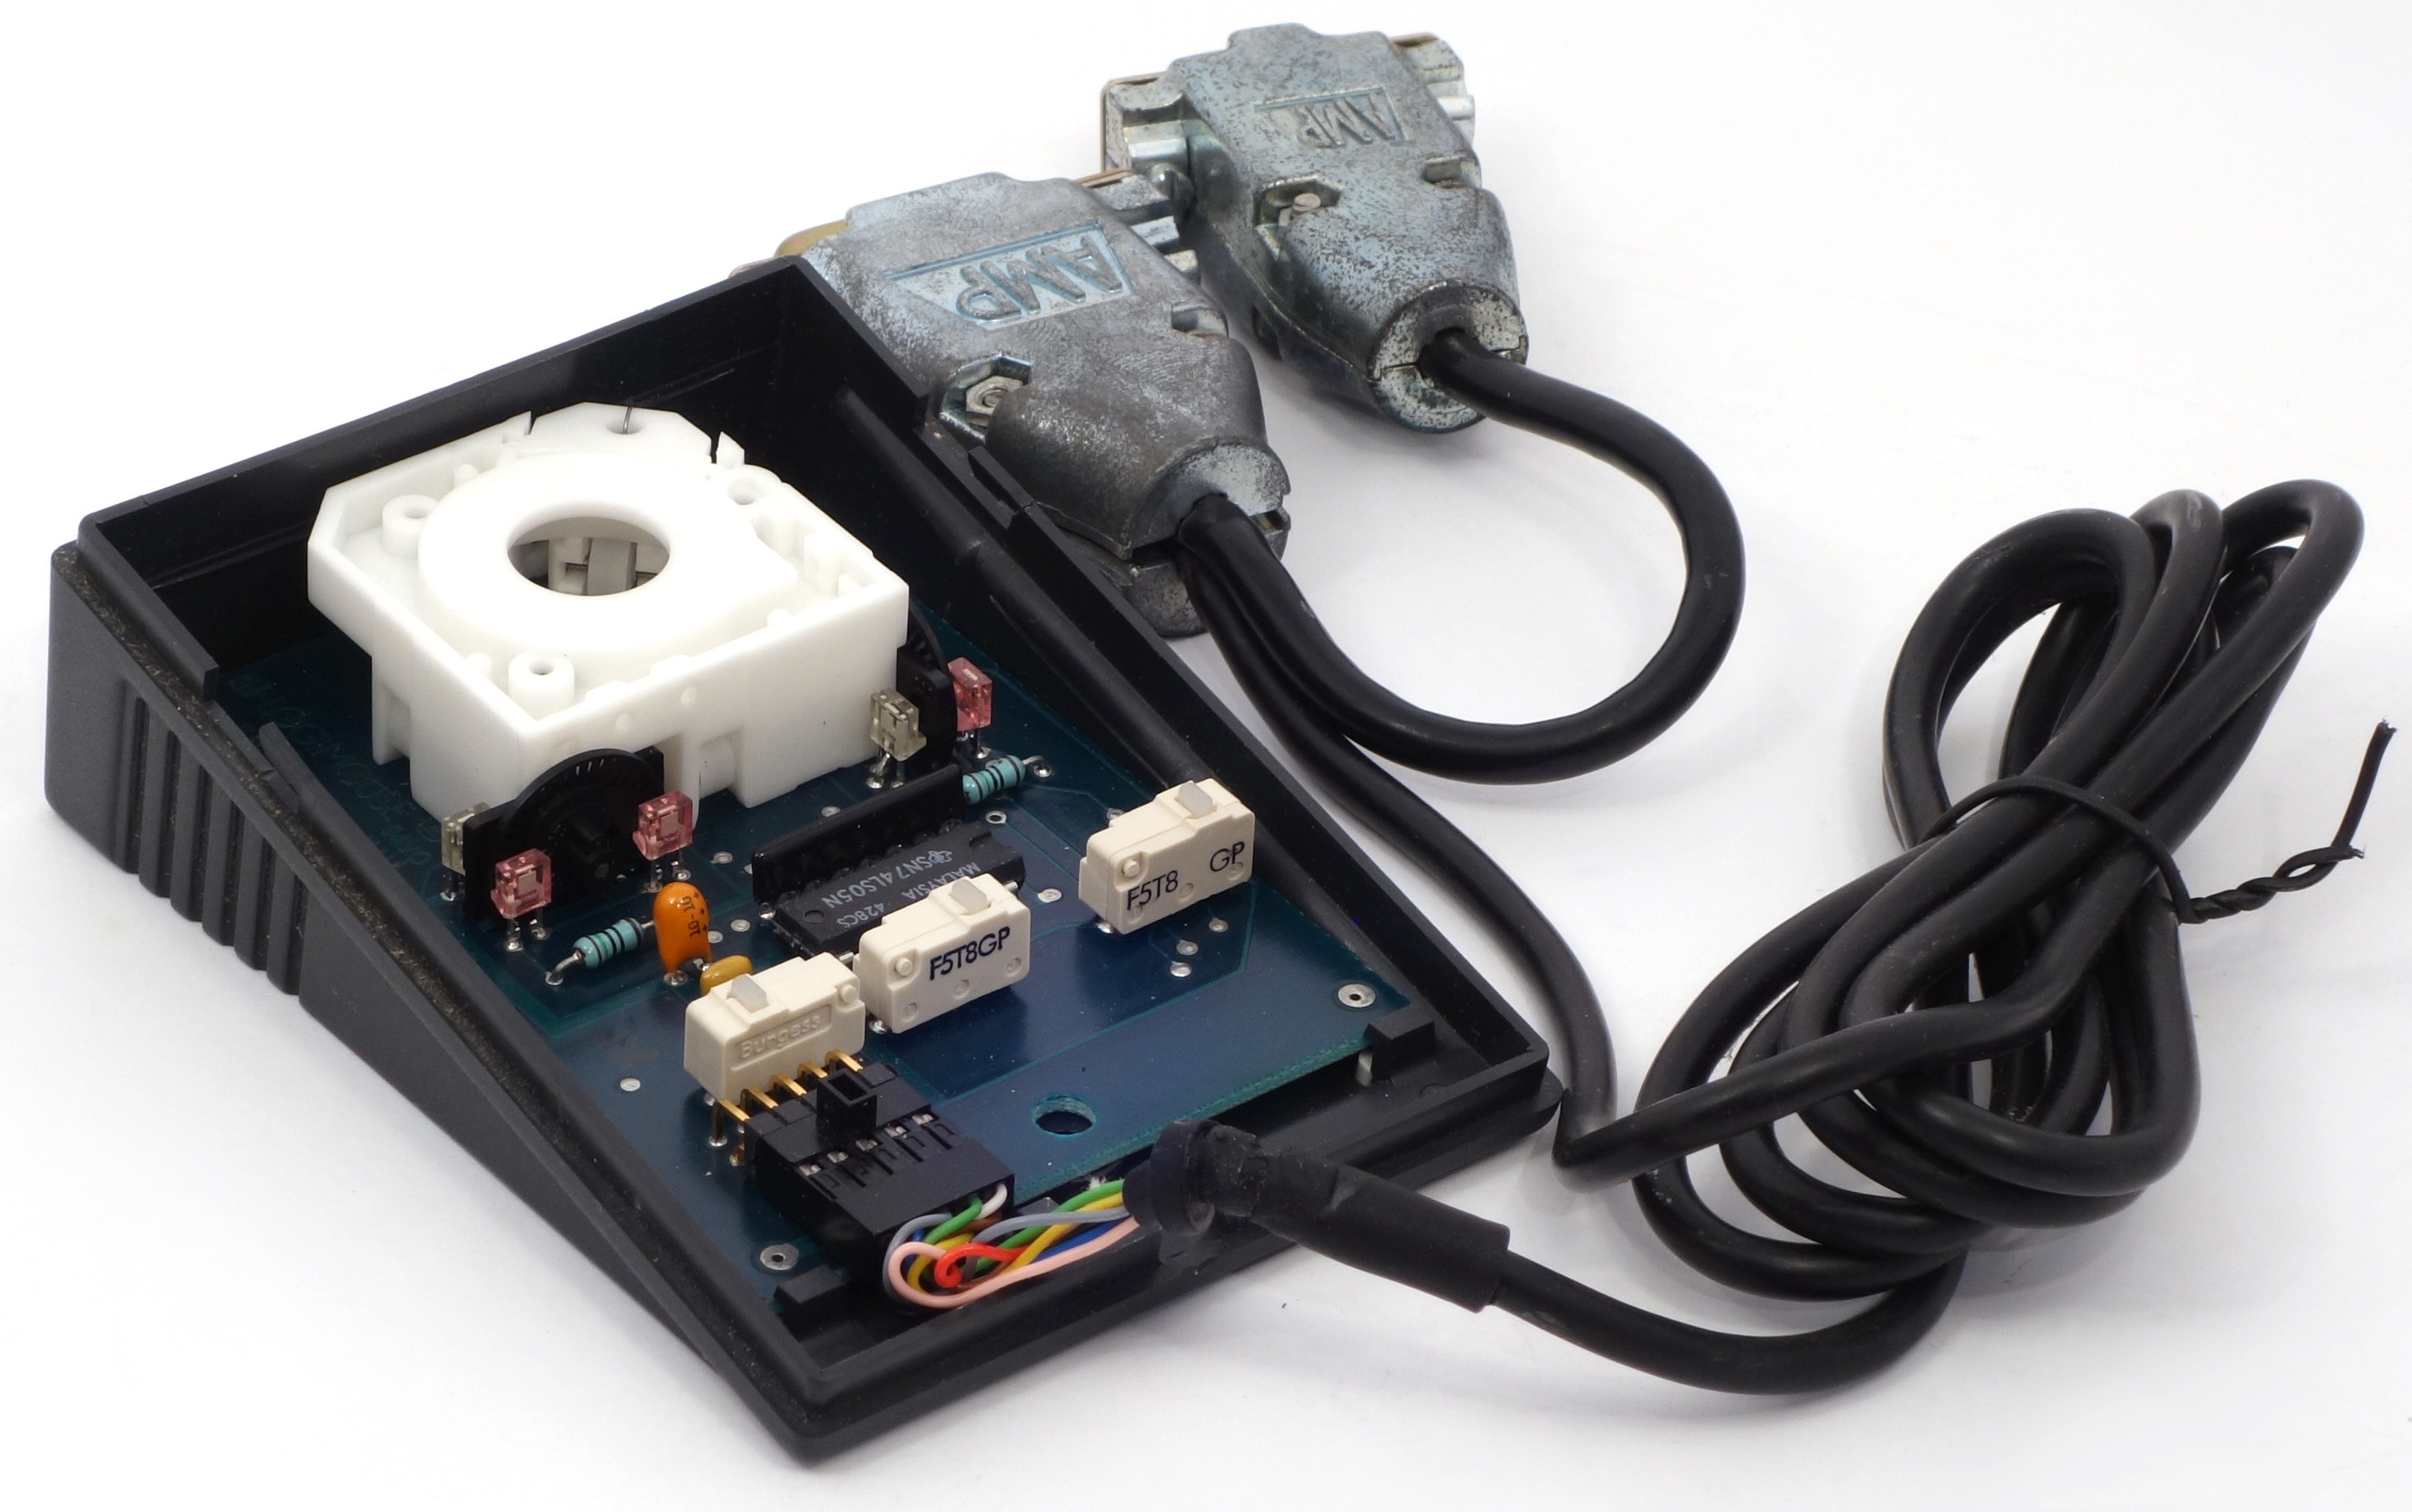
\includegraphics[scale=0.7]{1983_logitech_logimouse_p5/inside_30.jpg}
    \caption{LOGIMOUSE P5 disassembled}
    \label{fig:LogimouseP5Inside}
\end{figure}

The internal structure of the mouse is shown in fig. \ref{fig:LogimouseP5Inside}. The mouse uses optomechanical encoders.The optocouples and the optical interrupter disk are very similar to the corresponding parts in the mice of the 90-s (this can be considered one of the first such implementations). A distinctive feature of the encoder (as in P4 model) is an additional fixed mask that reduces the area of flare.

\begin{thebibliography}{9}
\bibitem {logimouse} J. Taylor. Faster then a speeding cursor key. // PC Magazine, V. 3, No. 2, February 7, 1984. - p. 243-245 \url{https://archive.org/details/PC-Mag-1984-02-07/page/n243/mode/2up}
\bibitem {futurenet} M. Holley. Logitech Logimouse Cable 1983 \url{https://commons.wikimedia.org/wiki/File:Logitech_Logimouse_Cable_1983.jpg}
\end{thebibliography}
\end{document}
